\chapter{Non-Disclosure Agreement}

\label{nda}

To ensure that all information, data, and materials accessed during the development of the application be kept confidential and will not be disclosed to any unauthorized parties, the developers/researchers have accomplished a signed Non-Disclosure agreement (NDA) to the Management Information System (MIS) as well as the Human Resource Mangement Office (HRMO). 

By signing this agreement, all involved parties commit to maintaining the confidentiality of the HRIS and MIS data, protecting it from any unauthorized use or distribution. These involved personnel are the Developers, MIS Director, HR, DCS Chair, and DCS Dean.

\begin{figure}[H]
    \centering
    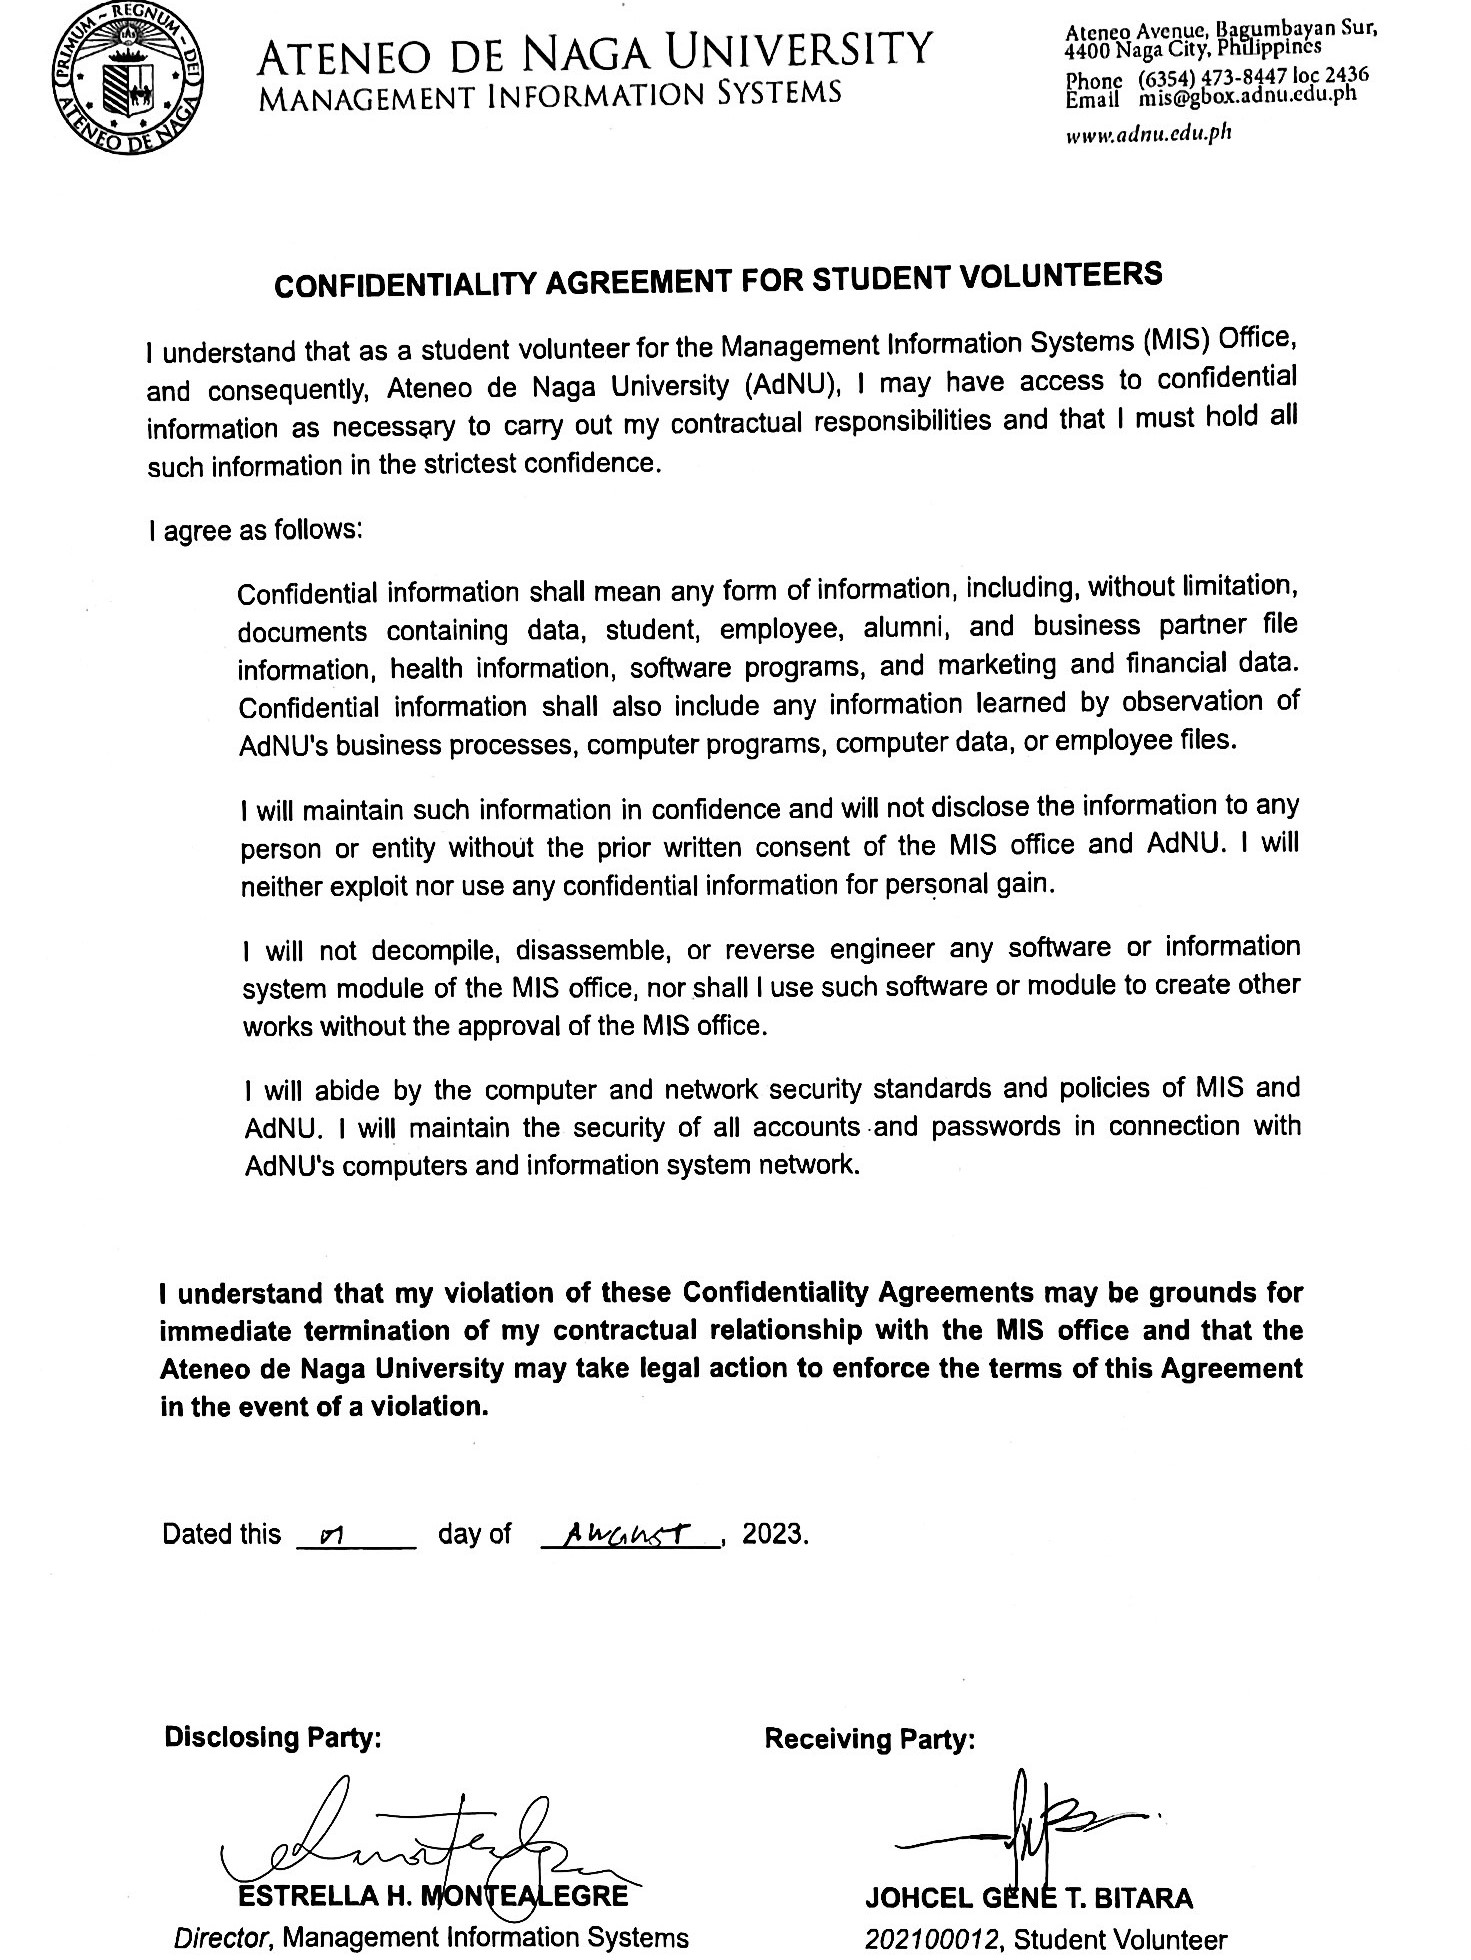
\includegraphics[width=1\textwidth]{figures/images/nda/mis-nda-bitara.JPG}
    \caption{MIS Confidentiality Agreement for Student Volunteers - Bitara}
    \label{fig:mis-nda-bitara}
\end{figure}

\begin{figure}[H]
    \centering
    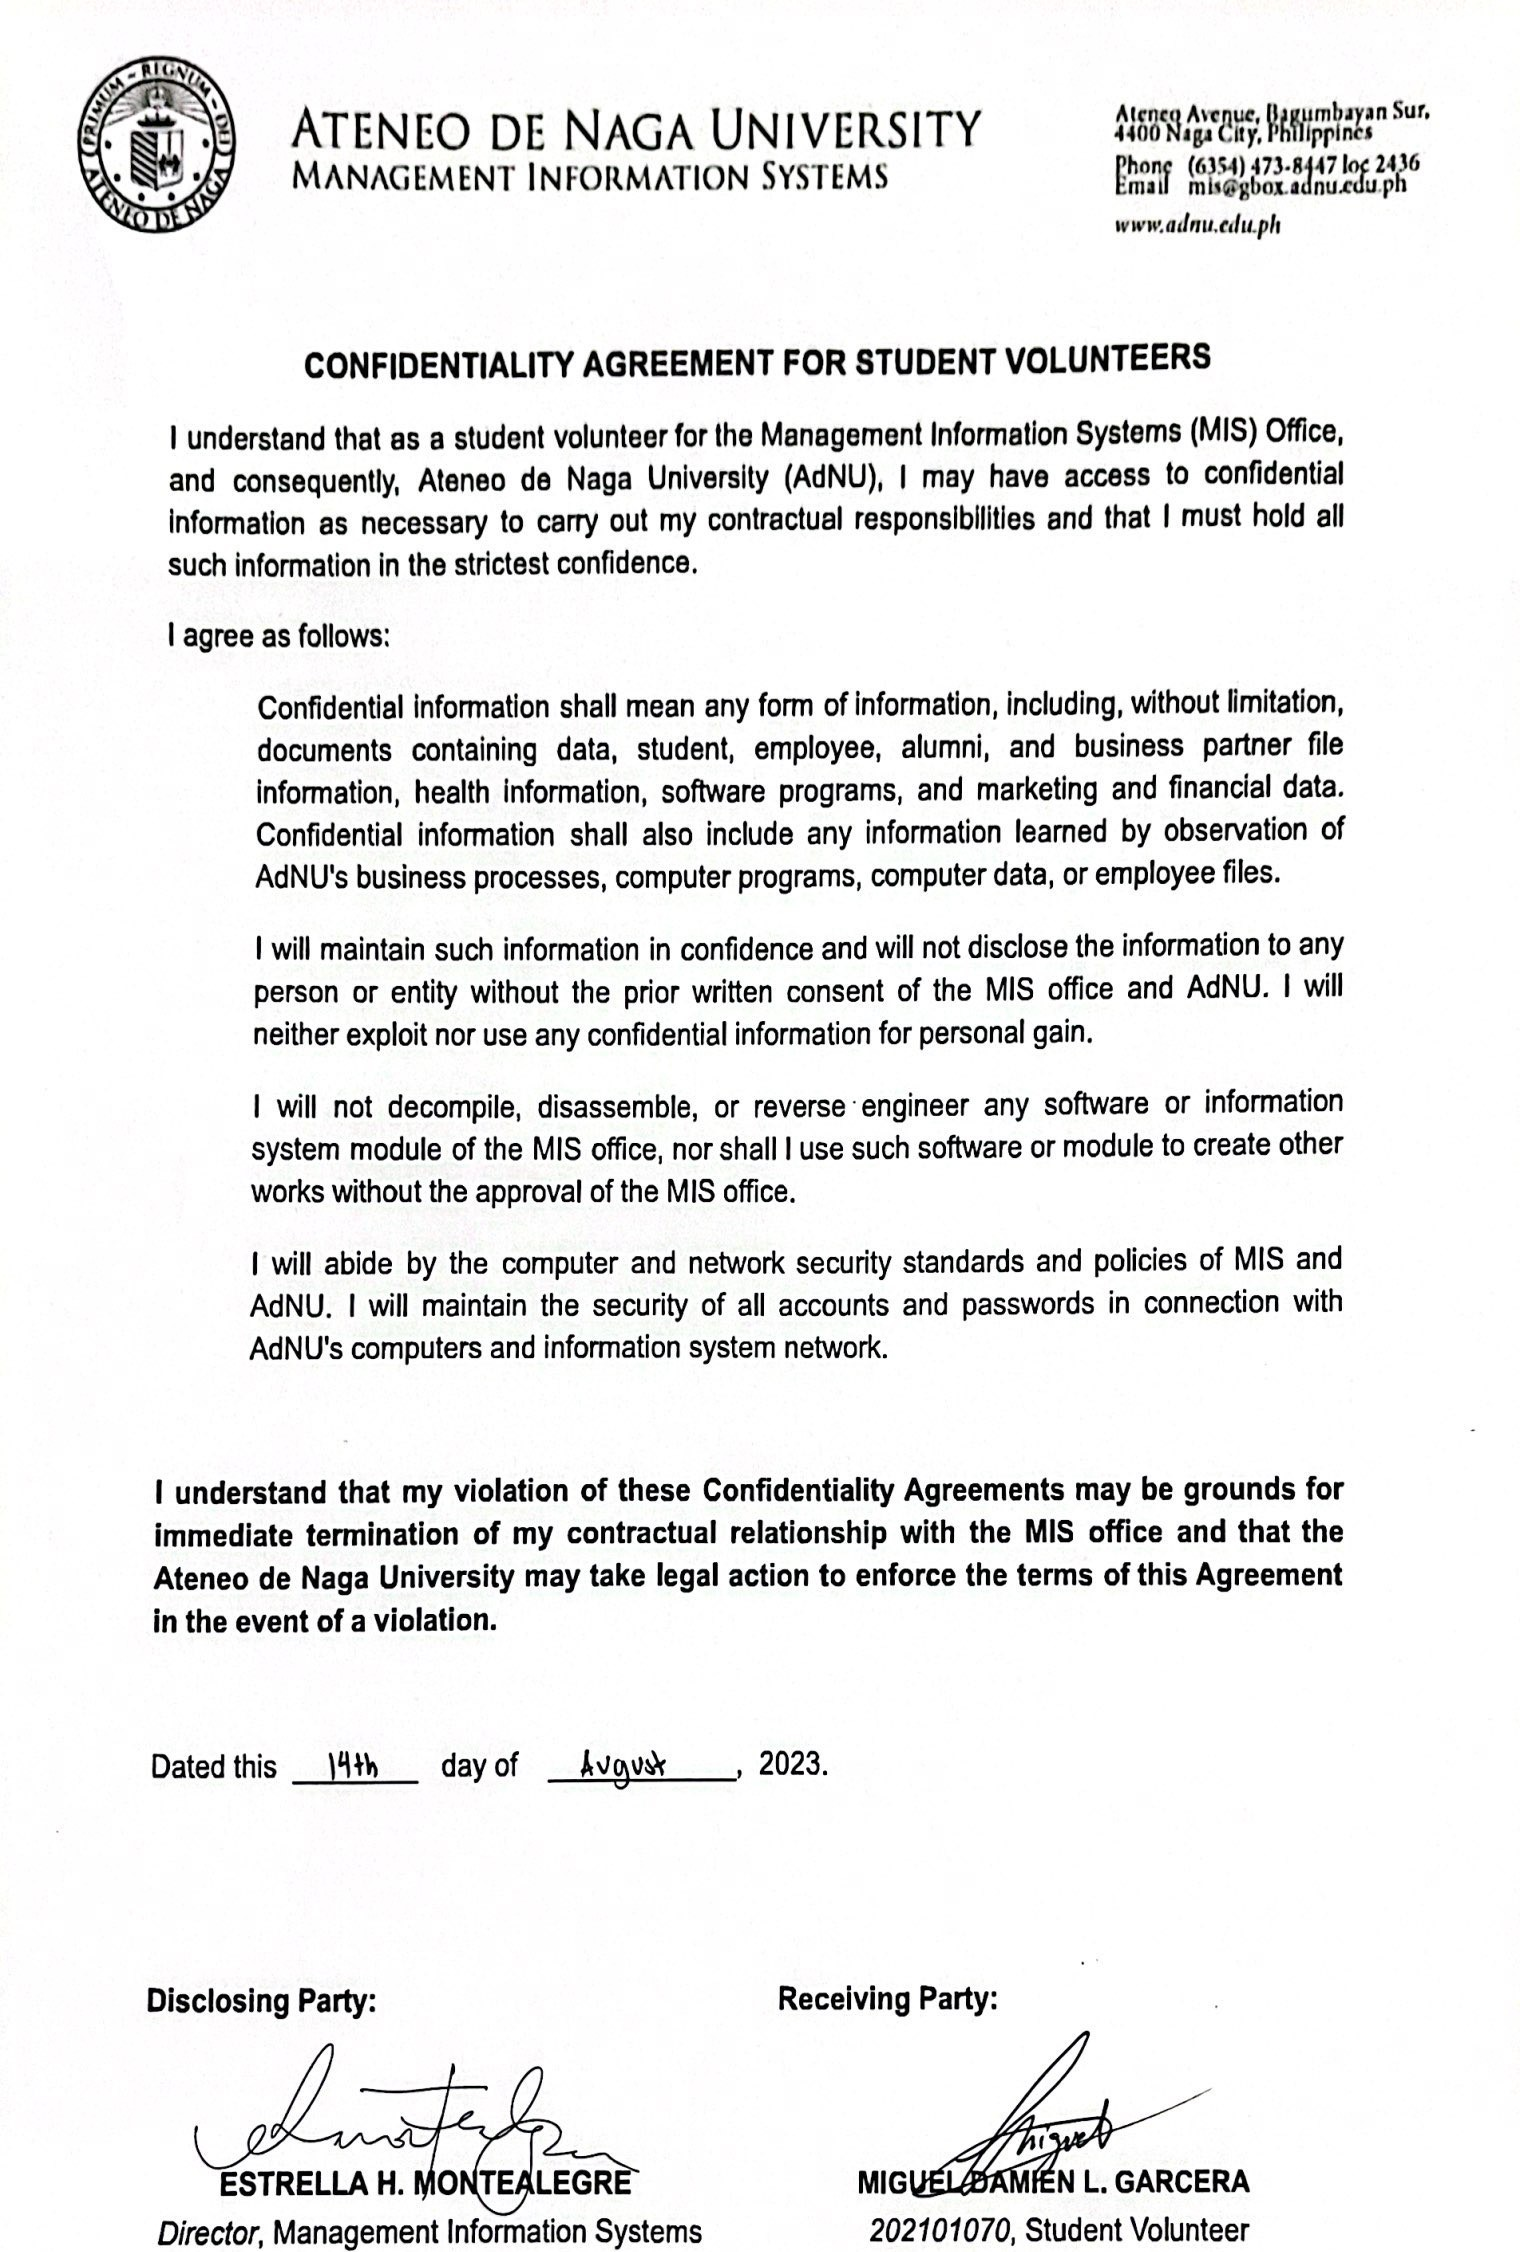
\includegraphics[width=0.95\textwidth]{figures/images/nda/mis-nda-garcera.JPG}
    \caption{MIS Confidentiality Agreement for Student Volunteers - Garcera}
    \label{fig:mis-nda-garcera}
\end{figure}

\begin{figure}[H]
    \centering
    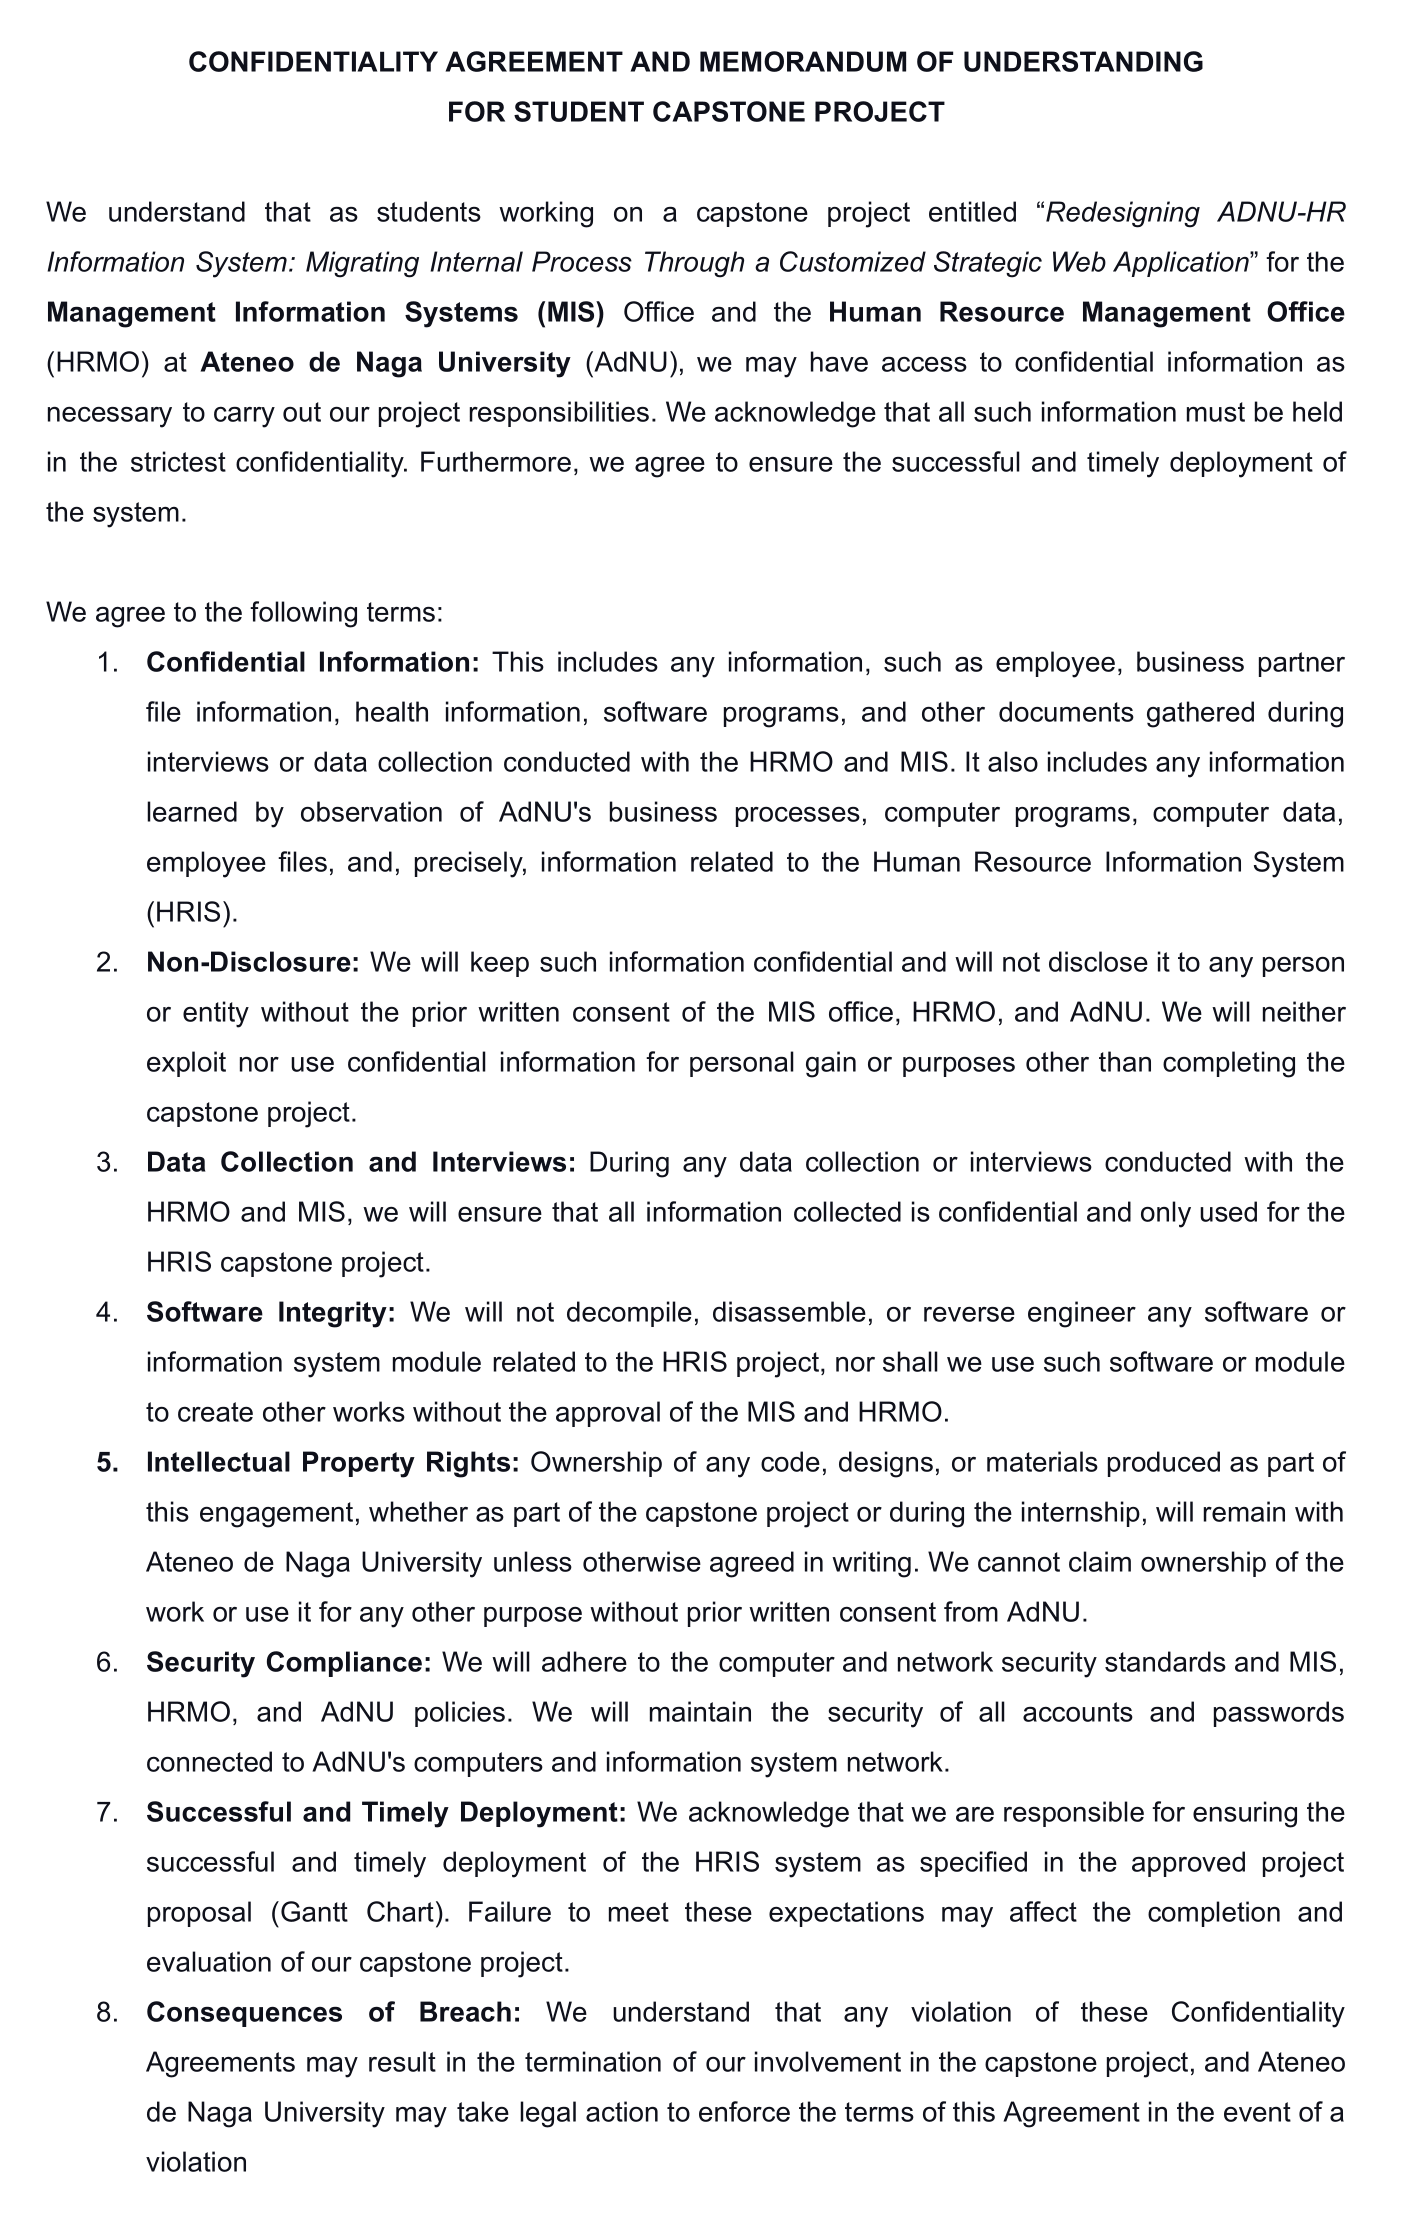
\includegraphics[width=0.9\textwidth]{figures/images/nda/hr-nda-1.png}
    \caption{HRMO Confidentiality Agreement and Memorandum of Understanding Page 1}
    \label{fig:hr-nda-1}
\end{figure}

\begin{figure}[H]
    \centering
    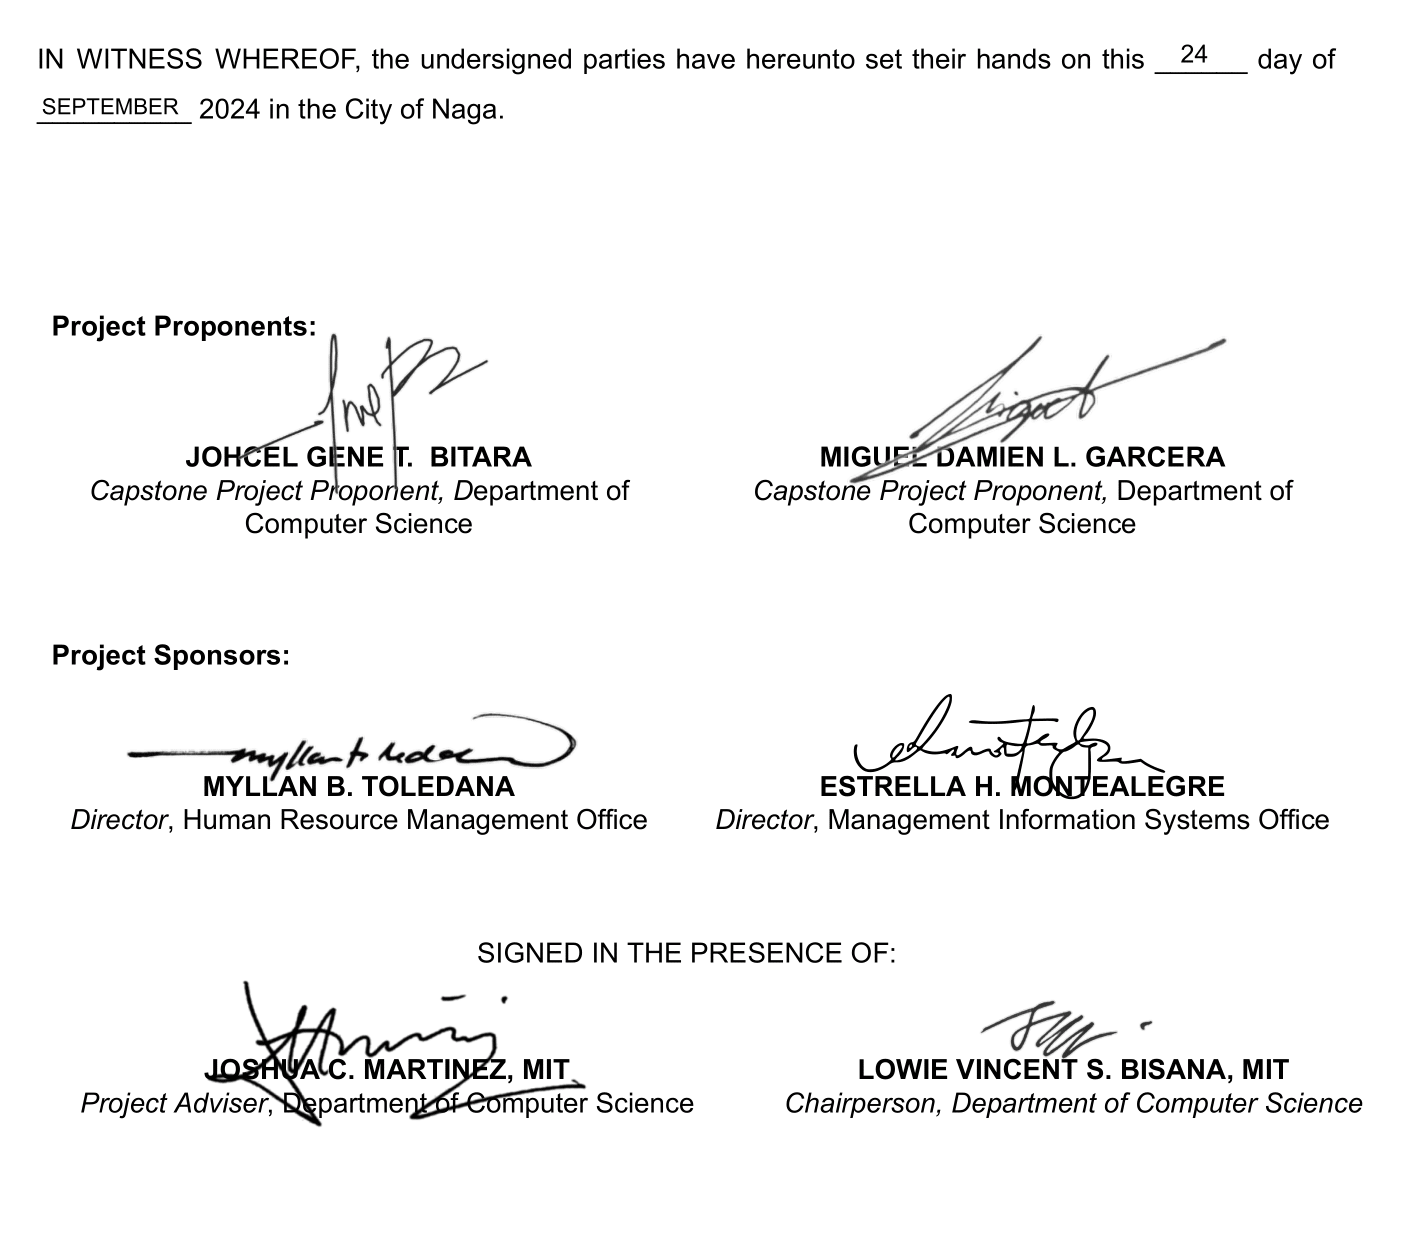
\includegraphics[width=1\textwidth]{figures/images/nda/hr-nda-2.png}
    \caption{HRMO Confidentiality Agreement and Memorandum of Understanding Page 2}
    \label{fig:hr-nda-2}
\end{figure}